% !TEX program = pdflatex
% !TEX TS-program = pdflatex
% !TEX encoding = UTF-8 Unicode
\documentclass[letterpaper, 10 pt, conference]{ieeeconf}
\usepackage{graphicx}
\overrideIEEEmargins
\IEEEoverridecommandlockouts

\usepackage[utf8]{inputenc}
\usepackage[T1]{fontenc}
\usepackage{amsmath}
\usepackage{amssymb}
\usepackage{booktabs}
\usepackage{multirow}
\usepackage{microtype}
\usepackage{etoolbox}

% Rótulos en español (ieeeconf.cls los fija en inglés)
\makeatletter
\def\fnum@table{TABLA~\thetable}
\patchcmd{\thebibliography}{\section*{References}}{\section*{Referencias}}{}{}
\patchcmd{\thebibliography}{{References}}{{Referencias}}{}{}
\makeatother

\setlength{\textfloatsep}{2pt plus 1pt minus 1pt}
\setlength{\floatsep}{2pt plus 1pt minus 1pt}
\setlength{\intextsep}{2pt plus 1pt minus 1pt}
\setlength{\abovecaptionskip}{1.2pt}
\setlength{\belowcaptionskip}{0pt}
\setcounter{topnumber}{4}
\setcounter{bottomnumber}{4}
\setcounter{totalnumber}{6}
\renewcommand{\topfraction}{0.95}
\renewcommand{\bottomfraction}{0.95}
\renewcommand{\textfraction}{0.05}
\renewcommand{\floatpagefraction}{0.90}
\renewcommand{\baselinestretch}{0.92}
\IEEEaftertitletext{\vspace{-1.3\baselineskip}}
\makeatletter
\def\section{\@startsection{section}{1}{\z@}{0.60ex plus 0.15ex minus 0.1ex}{0.15ex plus 0.05ex minus 0ex}{\normalfont\normalsize\centering\scshape}}
\makeatother
\emergencystretch=1.5em

\title{\LARGE \bf
Clasificación Multi-Clase de Artículos de Noticias de la BBC mediante el Ajuste Fino de Modelos Transformer Preentrenados
}

\author{Otto Wilmer Castillo Santacruz, Edgar Andrés Pérez Mora y Silvio Yopasa Romero\\
\textit{Maestría en Inteligencia Artificial (MAIA), Universidad de los Andes, Bogotá, Colombia}\\
{\tt\small \{o.castillos, ea.perezm1, s.yopasa\}@uniandes.edu.co}
}

\begin{document}

\maketitle
\thispagestyle{empty}
\pagestyle{empty}

%%%%%%%%%%%%%%%%%%%%%%%%%%%%%%%%%%%%%%%%%%%%%%%%%%%%%%%%%%%%%%%%%%%%%%%%%%%%%%%%
\section{Introducción}

La clasificación temática de artículos periodísticos en categorías editoriales (\textit{business}, \textit{entertainment}, \textit{politics}, \textit{sport} y \textit{tech}) es un problema clave del procesamiento de lenguaje natural \cite{c1}. Su relevancia radica en automatizar la indexación de repositorios digitales, el enrutamiento de noticias y el monitoreo de medios. Esta tarea es compleja porque muchos reportajes cruzan fronteras interdisciplinarias (p.~ej., regulación estatal del comercio electrónico o impacto financiero del delito digital), donde las bolsas de palabras fallan al ignorar el contexto sintáctico.

En el aprendizaje profundo, los modelos \textit{Transformer} \cite{c2} superaron el procesamiento secuencial de las redes recurrentes mediante la autoatención multicabeza, que relaciona simultáneamente cualquier par de términos del texto. Los codificadores bidireccionales preentrenados como BERT \cite{c3} y RoBERTa \cite{c4} sintetizan el contexto semántico global en el vector \texttt{[CLS]}. A su vez, modelos comprimidos por destilación como DistilBERT \cite{c5} retienen el $97\,\%$ de la capacidad de BERT con un $40\,\%$ menos de parámetros, mitigando el sobreajuste en corpus moderados.

El objetivo de este trabajo es desarrollar y validar un sistema reproducible de clasificación multi-clase con activación \textit{softmax} sobre el corpus de noticias de la BBC \cite{c1}. El enfoque comprende: (i) depuración, deduplicación y tokenización en subpalabras; (ii) comparación controlada en validación de cinco configuraciones (línea base léxica TF-IDF, BERT congelado y ajuste fino de DistilBERT, BERT y RoBERTa); (iii) reentrenamiento del modelo ganador sobre el conjunto de entrenamiento completo; y (iv) evaluación cuantitativa, por categoría y cualitativa en prueba independiente ($n = 319$), logrando $97.49\,\%$ de exactitud y $97.41 \pm 1.63\,\%$ de \textit{Macro F1}.

%%%%%%%%%%%%%%%%%%%%%%%%%%%%%%%%%%%%%%%%%%%%%%%%%%%%%%%%%%%%%%%%%%%%%%%%%%%%%%%%
\section{Metodología}

\textbf{Conjunto de datos y preprocesamiento.}
Se utilizó el corpus original de noticias de la BBC de Greene y Cunningham \cite{c1} ($2\,225$ artículos entre $2004$ y $2005$), descargado de su repositorio público en Kaggle \cite{c6}. No se hallaron valores nulos ni etiquetas contradictorias, pero se detectaron $101$ artículos duplicados ($98$ exactos y $3$ tras normalizar espacios y minúsculas). Su remoción previa fue esencial para evitar fuga de información entre particiones. El corpus único consta de $N = 2\,124$ textos en cinco clases con desbalance moderado (razón $1.47\times$): \textit{business} ($503$, $23.68\,\%$), \textit{sport} ($502$, $23.63\,\%$), \textit{politics} ($403$, $18.97\,\%$), \textit{entertainment} ($369$, $17.37\,\%$) y \textit{tech} ($347$, $16.34\,\%$).

Se estandarizaron espacios y saltos de línea conservando puntuación, dígitos y conectores (\textit{stopwords}), pues la autoatención requiere la estructura gramatical completa. Cada texto se codificó en subpalabras (\textit{WordPiece} de $30\,522$ términos en BERT y DistilBERT \cite{c3, c5}; \textit{Byte-Pair Encoding} de $50\,265$ términos en RoBERTa \cite{c4}), agregando los tokens \texttt{[CLS]} y \texttt{[SEP]} y la máscara binaria que ignora el relleno \texttt{[PAD]}.

La longitud presentó una media de $437.3 \pm 260.4$ subpalabras (mediana $381$). Aunque el límite de $512$ tokens de BERT cubre el $82.99\,\%$ de los tokens, el costo de la autoatención crece cuadráticamente con la longitud, $\mathcal{O}(L^2)$ \cite{c2}. Dado que en las noticias el titular y los primeros párrafos concentran la tesis principal, se fijó $\text{MAX\_LEN} = 256$ tokens, reduciendo en un $75\,\%$ el costo cuadrático de atención.

\textbf{Partición y protocolo experimental.}
El corpus depurado ($2\,124$ textos) se dividió estratificadamente (semilla $42$) en \texttt{Train} ($70\,\%$, $1\,486$), \texttt{Val} ($15\,\%$, $319$) y \texttt{Test} ($15\,\%$, $319$). Para aislar la selección de arquitectura de la prueba final, los cinco modelos candidatos se entrenaron sobre un subconjunto interno estratificado del $30\,\%$ de \texttt{Train} ($n = 445$) por $3$ épocas (paciencia $1$) y se evaluaron en el $100\,\%$ de \texttt{Val} ($n = 319$). El modelo ganador en \textit{Val Macro F1} se reentrenó sobre el $100\,\%$ de \texttt{Train} ($n = 1\,486$) hasta por $4$ épocas (paciencia $1$), conservando el mejor estado en \texttt{Val}. El conjunto \texttt{Test} ($n = 319$) se mantuvo reservado para una única evaluación final.

\textbf{Arquitecturas, pérdida y optimización.}
En cada codificador de $N_L$ capas y dimensión $d = 768$, cada cabezal de autoatención pondera el contexto por producto punto escalado, $\text{Atención}(Q, K, V) = \text{softmax}(QK^\top/\sqrt{d_k})V$ con $d_k = 64$ \cite{c2}. El vector final del primer token, $\mathbf{h}_{\texttt{[CLS]}} \in \mathbb{R}^{768}$, pasa por regularización (\textit{dropout} $0.1\text{--}0.2$) y una capa lineal ($\mathbb{R}^{768} \to \mathbb{R}^5$) que genera los \textit{logits} $\mathbf{z} = (z_1, \dots, z_5)$. La función \textit{softmax} calcula las probabilidades $p_c = e^{z_c}/\sum_{j=1}^5 e^{z_j}$, minimizando la pérdida de entropía cruzada categórica:
\begin{equation}
\mathcal{L}(\mathbf{z}, y) = -\log p_y = -z_y + \log\sum_{j=1}^{5} e^{z_j}
\label{eq:ce}
\end{equation}
Se evaluaron cinco modelos: (1) línea base TF-IDF (unigramas y bigramas hasta $30\,000$ términos ajustados solo en \texttt{Train}) con regresión logística multinomial; (2) BERT congelado ($12$ capas fijas, entrenando solo los $3\,845$ parámetros de la cabeza lineal con $\eta = 10^{-3}$); y el ajuste fino completo ($\eta = 2\times 10^{-5}$) de (3) DistilBERT ($6$ capas, $67.0\text{ M}$ de parámetros) \cite{c5}, (4) BERT-base ($12$ capas, $109.5\text{ M}$) \cite{c3} y (5) RoBERTa-base ($12$ capas, $85.5\text{ M}$ entrenables tras fijar la tabla BPE) \cite{c4}. Se utilizó Adam con decaimiento de pesos desacoplado ($\lambda = 0.01$) \cite{c7}, calentamiento lineal del $10\,\%$, lote efectivo de $16$, recorte de gradiente ($\|\nabla\|_2 \le 1.0$) y precisión mixta de $16$ bits. Se reportan Exactitud, Precisión Macro, Sensibilidad Macro y \textit{Macro F1} con la desviación estándar ($\pm\text{DE}$) entre las cinco clases para evaluar el equilibrio frente al desbalance.

%%%%%%%%%%%%%%%%%%%%%%%%%%%%%%%%%%%%%%%%%%%%%%%%%%%%%%%%%%%%%%%%%%%%%%%%%%%%%%%%
\section{Resultados}

\textbf{Comparación cuantitativa de modelos en Validación.}
La Tabla~\ref{tab:comparacion_val} muestra el desempeño en \texttt{Val} ($n = 319$) de los cinco modelos entrenados con el $30\,\%$ de \texttt{Train} ($n = 445$). El codificador BERT congelado obtuvo el desempeño más bajo (\textit{Macro F1} de $44.16 \pm 17.65\,\%$ y pérdida de $1.4173$), probando que el estado \texttt{[CLS]} preentrenado sin ajustar no discrimina directamente las cinco categorías. Al habilitar el ajuste fino del codificador, los tres \textit{transformers} superaron el $96.6\,\%$. \textbf{DistilBERT con ajuste fino} lideró con $98.12 \pm 1.42\,\%$ de \textit{Macro F1} ($98.12\,\%$ de exactitud), superando a RoBERTa ($97.02\,\%$), BERT ($96.62\,\%$) y la línea base TF-IDF ($94.96\,\%$).

\begin{table}[t]
\centering
\caption{Comparación en \texttt{Val} ($n = 319$) de modelos entrenados con el $30\,\%$ estratificado de \texttt{Train} ($n = 445$, $3$ épocas, semilla $42$). \textit{Macro F1 $\pm$ DE} indica media y desviación estándar entre las $5$ clases.}
\label{tab:comparacion_val}
\renewcommand{\arraystretch}{0.98}
\setlength{\tabcolsep}{4.0pt}
\resizebox{8.6cm}{!}{
\begin{tabular}{lcccc}
\toprule
\textbf{Modelo / Configuración} & \textbf{Parám. Entr.} & \textbf{Val Loss} & \textbf{Val Acc (\%)} & \textbf{Val Macro F1 $\pm$ DE (\%)} \\
\midrule
1. TF-IDF + Reg. Logística & $150.0\text{ k}$ & $0.8565$ & $94.98$ & $94.96 \pm 1.12$ \\
2. BERT congelado (\texttt{[CLS]} + lineal) & $3.8\text{ k}$ & $1.4173$ & $50.16$ & $44.16 \pm 17.65$ \\
3. \textbf{DistilBERT (ajuste fino)} & $\mathbf{67.0\text{ M}}$ & $0.5228$ & $\mathbf{98.12}$ & $\mathbf{98.12 \pm 1.42}$ \\
4. BERT-base (ajuste fino) & $109.5\text{ M}$ & $0.6068$ & $96.55$ & $96.62 \pm 3.06$ \\
5. RoBERTa-base (ajuste fino) & $85.5\text{ M}$ & $\mathbf{0.1695}$ & $97.18$ & $97.02 \pm 2.37$ \\
\bottomrule
\end{tabular}}
\end{table}

\textbf{Convergencia y desempeño por categoría en Prueba.}
Al reentrenar DistilBERT con el $100\,\%$ de \texttt{Train} ($n = 1\,486$, $4$ épocas), la pérdida en \texttt{Val} bajó de $0.2470$ (época $1$) a $0.0708$ (época $3$), alcanzando $98.78 \pm 1.16\,\%$ de \textit{Val Macro F1} ($98.75\,\%$ de exactitud) y activando la parada temprana tras la época $4$ (Fig.~\ref{fig:quant_eval}(b)), superando el $98.11 \pm 1.72\,\%$ de TF-IDF en \texttt{Val}.

\begin{table}[!t]
\centering
\caption{Desempeño por categoría en \texttt{Test} ($n = 319$) de DistilBERT ($100\,\%$ de \texttt{Train}) frente a TF-IDF, ordenado de mayor a menor F1-Score.}
\label{tab:test_categorias}
\renewcommand{\arraystretch}{0.95}
\setlength{\tabcolsep}{3.6pt}
\resizebox{8.6cm}{!}{
\begin{tabular}{lccccc}
\toprule
\textbf{Categoría (Soporte)} & \textbf{TP / FN / FP} & \textbf{Precisión (\%)} & \textbf{Sensibilidad (\%)} & \textbf{F1 DistilBERT (\%)} & \textbf{F1 TF-IDF (\%)} \\
\midrule
\textbf{sport} ($75$) [Mejor] & $75\ /\ 0\ /\ 0$ & $\mathbf{100.00}$ & $\mathbf{100.00}$ & $\mathbf{100.00}$ & $100.00$ \\
\textbf{entertainment} ($55$) & $53\ /\ 2\ /\ 0$ & $\mathbf{100.00}$ & $96.36$ & $98.15$ & $99.10$ \\
\textbf{politics} ($61$) & $58\ /\ 3\ /\ 0$ & $\mathbf{100.00}$ & $95.08$ & $97.48$ & $98.33$ \\
\textbf{business} ($76$) & $74\ /\ 2\ /\ 4$ & $94.87$ & $97.37$ & $96.10$ & $98.68$ \\
\textbf{tech} ($52$) [Menor F1] & $51\ /\ 1\ /\ 4$ & $92.73$ & $98.08$ & $95.33$ & $97.14$ \\
\midrule
\textbf{Macro $\pm$ DE / Exactitud} & $311\ /\ 8\ /\ 8$ & $\mathbf{97.52 \pm 3.11}$ & $\mathbf{97.38 \pm 1.65}$ & $\mathbf{97.41 \pm 1.63\ /\ 97.49}$ & $98.65 \pm 0.94$ \\
\bottomrule
\end{tabular}}
\end{table}

\begin{figure}[!t]
\centering
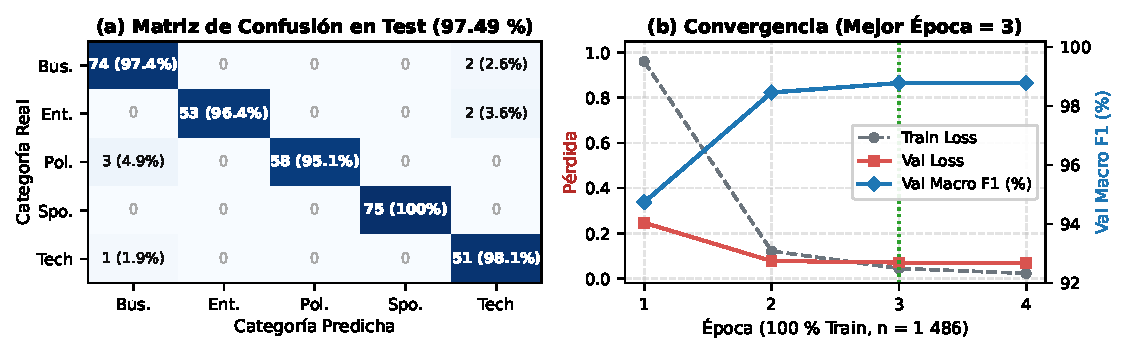
\includegraphics[width=0.96\linewidth]{figs/mp3_quant_eval.pdf}
\caption{Evaluación del modelo final: (a) Matriz de confusión en \texttt{Test} ($n = 319$, exactitud $97.49\,\%$); (b) Curvas de pérdida y \textit{Val Macro F1} ($100\,\%$ de \texttt{Train}), con punto óptimo en la época $3$.}
\label{fig:quant_eval}
\end{figure}

En la prueba independiente \texttt{Test} ($n = 319$, Tabla~\ref{tab:test_categorias} y Fig.~\ref{fig:quant_eval}(a)), DistilBERT logró \textbf{exactitud de $97.49\,\%$} ($311/319$, $8$ errores), \textbf{Precisión Macro de $97.52\,\%$}, \textbf{Sensibilidad Macro de $97.38\,\%$}, \textbf{\textit{Macro F1} de $97.41 \pm 1.63\,\%$} y pérdida de $0.1109$ ($4.4\times$ menor que el $0.4870$ de TF-IDF). Por clase, \textbf{\textit{sport}} fue la mejor con \textbf{$100.00\,\%$ en precisión, sensibilidad y F1} ($75/75$), seguida de \textit{entertainment} ($98.15\,\%$) y \textit{politics} ($97.48\,\%$); las tres obtuvieron $100.00\,\%$ de precisión ($0$ falsos positivos). En contraste, \textbf{\textit{tech}} tuvo el menor F1 ($95.33\,\%$) y precisión ($92.73\,\%$): pese a su alta sensibilidad ($98.08\,\%$, $51/52$), recibió $4$ falsos positivos de \textit{business} ($2$) y \textit{entertainment} ($2$). En textos completos ($\le 256$ tokens, $14.4\,\%$) logró $100.00\,\%$ de \textit{Macro F1}, frente a $97.13\,\%$ en truncados ($> 256$ tokens, $85.6\,\%$).

\textbf{Resultados cualitativos y geometría de representaciones.}
La Fig.~\ref{fig:qual_tsne} presenta la proyección t-SNE \cite{c8} de $\mathbf{h}_{\texttt{[CLS]}} \in \mathbb{R}^{768}$ en \texttt{Test}. El coeficiente de silueta coseno subió $4.2\times$, de $0.2062$ (congelado) a $0.8757$ tras el ajuste fino ($\Delta = +0.6695$; de $0.1159$ a $0.7233$ euclidiano), separando claramente las cinco clases.

\begin{figure}[!t]
\centering
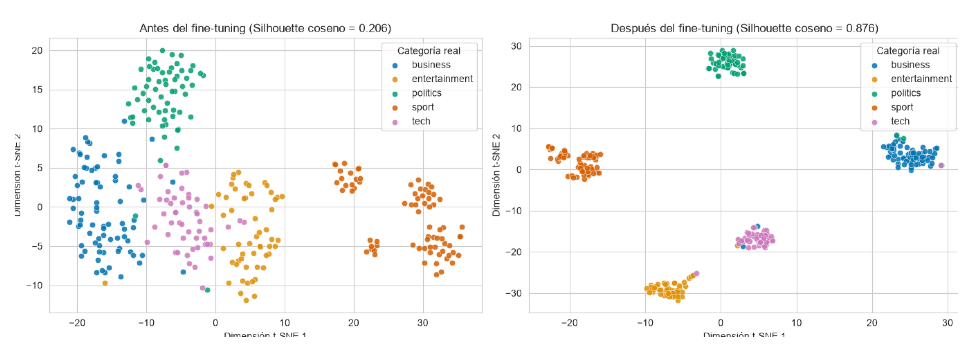
\includegraphics[width=0.96\linewidth]{figs/mp3_qual_eval.pdf}
\caption{Proyección t-SNE \cite{c8} de \texttt{[CLS]} ($\mathbb{R}^{768}$) en \texttt{Test} ($n = 319$): (izq.) preentrenado congelado ($\text{Sil.}_{\text{cos}} = 0.206$); (der.) DistilBERT ajustado ($\text{Sil.}_{\text{cos}} = 0.876$).}
\label{fig:qual_tsne}
\end{figure}

\begin{table}[!t]
\centering
\caption{Ejemplos reales del conjunto de prueba independiente (\texttt{Test}, $n = 319$): aciertos prototípicos y errores de frontera interdisciplinaria.}
\label{tab:cualitativo_test}
\renewcommand{\arraystretch}{0.95}
\setlength{\tabcolsep}{2.6pt}
\resizebox{8.6cm}{!}{
\begin{tabular}{llcl}
\toprule
\textbf{ID (Tokens)} & \textbf{Real $\to$ Pred.} & $\mathbf{P_{\text{pred}}\ (P_{\text{real}})}$ & \textbf{Fragmento en \texttt{Test} (términos clave en \textbf{negrita}) e interpretación} \\
\midrule
\texttt{\#213} ($302$) & \textit{bus.} $\to$ \textit{bus.} \checkmark & $99.01\,\%$ ($99.01\,\%$) & ``India's \textbf{Maruti} sees \textbf{profits jump}... \textbf{carmaker}'' (léxico financiero claro). \\
\texttt{\#75} ($913$) & \textit{spo.} $\to$ \textit{spo.} \checkmark & $98.93\,\%$ ($98.93\,\%$) & ``Irish \textbf{Athletics} Year... \textbf{Olympic champion}'' (acierto pese al truncado). \\
\texttt{\#312} ($284$) & \textit{pol.} $\to$ \textit{pol.} \checkmark & $98.52\,\%$ ($98.52\,\%$) & ``February \textbf{poll} claim... \textbf{election} campaign'' (vocabulario parlamentario). \\
\midrule
\texttt{\#62} ($1\,026$) & \textit{bus.} $\to$ \textit{tech} $\times$ & $97.95\,\%$ ($0.39\,\%$) & ``Making your \textbf{office} work... \textbf{gadgets}'' (apertura sobre equipos digitales). \\
\texttt{\#311} ($469$) & \textit{pol.} $\to$ \textit{bus.} $\times$ & $96.68\,\%$ ($1.93\,\%$) & ``\textbf{BAA} support ahead of \textbf{court}... \textbf{airport operator}'' (litigio corporativo). \\
\texttt{\#31} ($370$) & \textit{pol.} $\to$ \textit{bus.} $\times$ & $84.78\,\%$ ($1.10\,\%$) & ``UK \textbf{firms} embracing \textbf{e-commerce}... DTI'' (tesis política al cierre). \\
\texttt{\#246} ($287$) & \textit{ent.} $\to$ \textit{tech} $\times$ & $49.39\,\%$ ($45.59\,\%$) & ``\textbf{Download} chart delayed... \textbf{digital} music \textbf{singles}'' (duda calibrada). \\
\bottomrule
\end{tabular}}
\end{table}

En \texttt{Test}, los $311$ aciertos tuvieron mediana de confianza \textit{softmax} de $98.50\,\%$, y los $8$ errores mediana de $96.00\,\%$ (rango $[49.39\,\%, 97.95\,\%]$). La Tabla~\ref{tab:cualitativo_test} detalla ejemplos reales de \texttt{Test}. Por oclusión de tokens en \texttt{Test} (\textit{politics}, $P_{\text{base}} = 98.19\,\%$), ocultar ``\textit{lord}'' ($\Delta P = -0.24\text{ pp}$) o ``\textit{ministers}'' ($\Delta P = -0.15\text{ pp}$) redujo la probabilidad correcta, mientras que ``\textit{chancellor}'' ($\Delta P = +0.03\text{ pp}$) la elevó por su uso económico. En $5$ noticias externas inéditas (fuera del corpus), acertó $5/5$ ($P_{\text{pred}} \in [96.78\,\%, 98.80\,\%]$).

%%%%%%%%%%%%%%%%%%%%%%%%%%%%%%%%%%%%%%%%%%%%%%%%%%%%%%%%%%%%%%%%%%%%%%%%%%%%%%%%
\section{Discusión}

Los resultados explican tres aspectos metodológicos:
(i) \textbf{Rol del ajuste fino:} la mejora de $+53.96\text{ pp}$ en \textit{Macro F1} sobre BERT congelado ($98.12\,\%$ vs.~$44.16\,\%$) y el aumento de $4.2\times$ en silueta (Fig.~\ref{fig:qual_tsne}) prueban que el preentrenamiento \cite{c3} agrupa \texttt{[CLS]} por sintaxis general; solo al actualizar las matrices de atención ($W_Q, W_K, W_V$) se separan las clases editoriales.
(ii) \textbf{Capacidad y convergencia:} con $445$ textos, DistilBERT ($6$ capas, $67.0\text{ M}$) \cite{c5} superó a BERT ($109.5\text{ M}$) y RoBERTa ($85.5\text{ M}$ entrenables), pues su menor capacidad destilada reduce el riesgo de sobreajuste y converge más rápido en $3$ épocas.
(iii) \textbf{Contraste con TF-IDF y truncado:} DistilBERT superó a TF-IDF en \texttt{Val} con el $30\,\%$ ($+3.16\text{ pp}$) y el $100\,\%$ de \texttt{Train} ($98.78\,\%$ vs.~$98.11\,\%$), logrando una pérdida $4.4\times$ menor en \texttt{Test}. La leve ventaja de TF-IDF en \textit{Macro F1} de \texttt{Test} ($98.65\,\%$ vs.~$97.41\,\%$, $4$ artículos de $319$) se debe a que TF-IDF observa el $100\,\%$ de las palabras en textos largos, mientras que el \textit{transformer} lee solo los primeros $256$ tokens.

\textbf{Calibración, literatura y mejoras.}
Siete de los ocho errores de \texttt{Test} ocurrieron en textos largos ($324\text{--}1\,034$ tokens) con alta confianza ($84.78\text{--}97.95\,\%$), mostrando sobreconfianza cuando los primeros $256$ tokens destacan un ángulo secundario tecnológico o financiero. La exactitud ($97.49\,\%$ en $2\,124$ textos únicos) concuerda con la literatura del corpus BBC \cite{c1} y de DistilBERT \cite{c5}, evitando la inflación de métricas por los $101$ duplicados del corpus original. Como trabajo futuro se propone: (1) truncado inicio-final (\textit{head+tail}, primeros $192$ y últimos $64$ tokens); (2) ensamble de probabilidades DistilBERT + TF-IDF; y (3) suavizado de etiquetas ($\epsilon = 0.05$) para moderar la sobreconfianza en noticias de frontera.

\newpage
%%%%%%%%%%%%%%%%%%%%%%%%%%%%%%%%%%%%%%%%%%%%%%%%%%%%%%%%%%%%%%%%%%%%%%%%%%%%%%%%
\begin{thebibliography}{99}
\setlength{\itemsep}{0.2pt}
\setlength{\parskip}{0pt}

\bibitem{c1} D. Greene and P. Cunningham, ``Practical solutions to the problem of diagonal dominance in kernel document clustering,'' in \textit{Proc. 23rd Int. Conf. Mach. Learn. (ICML)}, 2006, pp. 377--384.

\bibitem{c2} A. Vaswani \textit{et al.}, ``Attention is all you need,'' in \textit{Adv. Neural Inf. Process. Syst. (NeurIPS)}, vol. 30, 2017, pp. 5998--6008.

\bibitem{c3} J. Devlin, M.-W. Chang, K. Lee, and K. Toutanova, ``BERT: Pre-training of deep bidirectional transformers for language understanding,'' in \textit{Proc. Conf. North Amer. Chapter Assoc. Comput. Linguistics (NAACL-HLT)}, 2019, pp. 4171--4186.

\bibitem{c4} Y. Liu \textit{et al.}, ``RoBERTa: A robustly optimized BERT pretraining approach,'' \textit{arXiv preprint arXiv:1907.11692}, 2019.

\bibitem{c5} V. Sanh, L. Debut, J. Chaumond, and T. Wolf, ``DistilBERT, a distilled version of BERT: smaller, faster, cheaper and lighter,'' in \textit{NeurIPS Workshop Energy Efficient Mach. Learn. Cogn. Comput. (EMC$^2$)}, 2019.

\bibitem{c6} J. Ferretti, ``BBC Articles Dataset,'' \textit{Kaggle Repository} (\texttt{jacopoferretti/\allowbreak bbc-articles-\allowbreak dataset}), 2023.

\bibitem{c7} I. Loshchilov and F. Hutter, ``Decoupled weight decay regularization,'' in \textit{Proc. Int. Conf. Learn. Represent. (ICLR)}, 2019.

\bibitem{c8} L. van der Maaten and G. Hinton, ``Visualizing data using t-SNE,'' \textit{J. Mach. Learn. Res. (JMLR)}, vol. 9, pp. 2579--2605, 2008.

\end{thebibliography}

\end{document}
